\documentclass[11pt, oneside]{book}
\usepackage{tfgstyle}

\title{Búsquedas de Materia Oscura Producida con Quarks top en el Experimento CMS}
\author{Nicolás Babío Elguero}
\date{Fecha}

\begin{document}


\frontmatter
\thispagestyle{empty}

\vspace{0.3cm}
\begin{figure}[H]
    \centering
    \includegraphics[height=2.3cm]{images/Logo-UCnuevo.png}
    \label{logo 50UC}
\end{figure}

\begin{center}
    \vspace{0.3cm}
    \huge
    Facultad

    de

    Ciencias

    \vspace{1.4cm}

    \huge
    \textbf{Búsquedas de Materia Oscura Producida con Quarks Top en el Experimento CMS}

    \vspace{0.3cm}
    \LARGE
    (Searches for Dark Matter Produced with Top Quarks in the CMS Experiement)

    \vspace{2cm}
    \Large
    Trabajo de Fin de Grado

    para acceder al
    \vspace{0.4cm}

    \textbf{GRADO EN FÍSICA}
    \vspace{2cm}
\end{center}

\begin{flushright}
    \Large
    \textbf{Autor: Nicolás Babío Elguero}

    \vspace{0.3cm}\textbf{
    Director: Jesús Manuel Vizán García}

    \vspace{0.3cm} \textbf{
    Fecha: }
\end{flushright}


\newpage{\ }
\thispagestyle{empty}

% Dedicatoria

\dedicatoria{Dedicatoria.}
\newpage{\ }
\thispagestyle{empty}

\chapter*{Resumen}
Resumen en español

\chapter*{Abstract}
Abstract in english

\newpage{\ }
\thispagestyle{empty}

% Indice
\chapter*{Índice}
\renewcommand{\contentsname}{}

\tableofcontents
\newpage{\ }
\thispagestyle{empty}

\mainmatter

\chapter{Introducción}


% OTRA SECCIÓN DISTINTA?

\section{Marco teórico}



Modelo estándar de partículas \\

Materia oscura --> Posibles candidatos, por qué se sabe que existe...

\section{Quarks top}

Hacer hincapié en los quarks top, explicar los canales de desintegración mostrar algún diagrama de feynmann de la desintegración en DM

\section{LHC}

Hablar sobre el CERN

Explicar qué es, por qué existe...\\

CMS --> Objetivo del experimento, detectores...




\chapter{Marco Teórico}

\section{Modelo Estándar de la Física de Partículas}

La física de partículas se fundamenta en lo que se conoce como el Modelo Estándar de la Física de Partículas. Ésta es una teoría que fue desarrollada durante la década de los años 70 por la comunidad científica gracias a los conocimientos previos que se tenían sobre la estructura de la materia, la mecánica cuántica y la relatividad general. El Modelo Estándar está fundamentado en la mecánica cuántica y en la teoría cuántica de campos y explica a la vez la cromodinámica cuántica (relacionada con la interacción nuclear fuerte) y la teoría electrodébil (relacionada con las interacciones electromagnéticas y débil). Sin embargo, falla en explicar la teoría de la relatividad general. \\

% ES IMPORTANTE ESTO? -->
El Modelo Estándar se fundamenta en las simetrías ya que determinan las interacciones y las propiedades de las partículas fundamentales. Esto nace del Teorema de Noether, que indica que a cada simetría continua y derivable de un sistema le corresponde una cantidad conservada. \cite{noether_th} Las simetrías que aparecen en el Modelo Estándar se conocen como simetrías gauge, que indica que la ecuaciones sean invariantes baja un tipo de transformaciones locales. Matemáticamente, el Modelo Estándar se define bajo el grupo de simetría $SU(3) \times SU(2)_L \times U(1)_Y$ que corresponde a la teoría de QCD y a la teoría electrodébil. Del grupo $U(1)_Y$, que es el correspondiente a la hipercarga débil, surge la conservación de carga eléctrica. Del grupo de interacción débil $SU(2)_L$ surge la conservación del isospin débil. Por último, del grupo de la interacción fuerte $SU(3)$ surge la conservación de la carga de color.\\

La teoría del Modelo Estándar defiende que existen un grupo de partículas que constituyen la materia, llamados fermiones, y de las que todo el universo es constituido y que interaccionan entre ellas gracias al intercambio de unas partículas llamadas bosones gauge. Vayamos desglosando poco a poco estas partículas:\\

 Como ya se ha mencionado, los fermiones son las partículas que forman toda la materia: desde las células hasta las estrellas. Los fermiones son 12 partículas con spin semientero (y sus correspondientes antipartículas) que se pueden dividir en dos grupos de 6 partículas: leptones y quarks. Los leptones son partículas fermiónicas sin carga de color. Este grupo se divide en tres subgrupos o generaciones: el electrón $e^-$ y neutrino electrónico $\nu_e$, el muón $\mu$ y el neutrino muónico $\nu_\mu$ y el tau $\tau$ y el neutrino tauónico $\nu_\tau$. El electrón, muón y tau tienen carga eléctrica negativa por lo que interactúan mediante la fuerza electromagnética además de la fuerza débil, mientras que los neutrinos son partículas de carga neutra que interactúan únicamente mediante la fuerza débil. Por otro lado se tienen los quarks, que son partículas con carga de color por lo que interacción mediante la fuerza fuerte. Se dividen en tres generaciones: quarks \textit{up} $u$ y \textit{down} $d$, \textit{charm} $c$ y \textit{strangeness} $s$, \textit{top} $t$ y \textit{bottom} $b$. Los quarks interactúan, aparte de mediante la fuerza fuerte, mediante la interacción electromagnética y la interacción débil. \\

 Por otro lado, los bosones de gauge son partículas con spin entero. Estas partículas son las que portan las fuerzas que sufren todas las partículas. Estos bosones son el fotón $\gamma$ que media la fuerza electromagnética, el gluón $g$ que media la fuerza fuerte y los bosones $W^+$, $W^-$ y $Z^0$ que median la fuerza débil, todos ellos con spin 1. Además, se tiene el bosón de Higgs $H^0$ que se asocia al mecanismo que da masa a las partículas.  \\

\textcolor{red}{EXPLICAR SIMETRÍAS}\\
Además, se explican a continuación las interacciones fundamentales que describe el modelo estándar:\\

De más fuerte a más débil, la \textbf{fuerza nuclear fuerte} surge de la simetría $SU(3)$ y es la responsable de que los nucleones se mantengan ligados en el núcleo. Los mediadores de esta fuerza son los gluones, partícula con masa nula pero que tienen carga de color, lo que les permite interactuar entre ellos. Este tipo de fuerza depende linealmente de la distancia, esto es, el acoplamiento de las partículas con carga de color aumenta con la distancia. Esto puede provocar que si dos quarks se separan mucho, la fuerza sea tan intensa que se produzca un gluón que decae en un par quark-antiquark que se recombinan con los quarks que existían inicialmente. Este es el principio fundamental del confinamiento de color y cuya consecuencia es la aparición de jets hadrónicos que son detectados por los experimentos del CERN. A continuación está la \textbf{fuerza nuclear débil}, siguiendo la simetría $SU(2)$ que se acopla a la parte leptónica del modelo estándar. Está mediada por tres bosones masivos, dos de ellos cargados, el $W^+$ y el $W^-$, y un bosón sin carga, el $Z^0$. El hecho de que los bosones tengan masa hace que sea de corta distancia y que las partículas que interactúan mediante esta fuerza decaigan muy rápidamente. Además, la interacción débil y la electromagnética están acopladas en los que se conoce como Teoría Electrodébil. La última interacción que describe el modelo estándar es la \textbf{interacción electromagnética}, regida por el grupo de simetría $U(1)$, actúa entre partículas con carga eléctrica. Su partícula mediadora, el fotón $\gamma$, no tiene masa por lo que el rango de esta interacción es infinito. Esta fuerza es la responsable de los fenómenos eléctricos y magnéticos que vivimos en el día a día. \\

Aunque no sea descrito por el Modelo Estándar, es de interés explicar la fuerza gravitatoria. Esta fuerza no está mediada por ninguna partícula sino que es la consecuencia de vivir en un Espacio-Tiempo que se curva debido a la presencia de materia. La gravedad tiene un papel fundamental en la búsqueda de la Materia Oscura ya que se sabe que interacciona mediante esta fuerza.\\

Por otro lado, y aunque no sea una fuerza fundamental, cabe destacar el mecanismo de Higgs que es el que provoca que las partículas adquieran masa. Esta teoría fue propuesta por Peter Higgs, Robert Brout y François Englert y predice la existencia de un campo que surge de la ruptura del grupo de simetría $SU(2)_LU(1)_Y$, correspondiente a la teoría electrodébil. Este campo, llamado campo de Higgs, interactúa con algunas partículas infiriéndoles masa. \textcolor{red}{REVISAR}

\section{Materia Oscura}

La búsqueda de Materia Oscura (DM por sus siglas en inglés, \textit{Dark Matter}) es uno de los proyectos más ambiciosos en el campo de la física actualmente. La materia oscura se predice que es casi 5 veces más abundante que la materia bariónica, que es el tipo de materia a la que estamos acostumbrados y que compone todo desde las estrellas hasta los núcleos de los átomos. El problema de detectar la materia oscura no nace de su abundancia, sino de que no interacciona mediante la fuerza electromagnética provocando que ni emita ni refleje luz. Por tanto, la tarea de detección de este tipo de materia es muy compleja y la mayoría de las veces se tiene que inferir de efectos gravitaciones sobre la materia bariónica.\\

Aunque este tipo de materia no pueda ser detectada de manera directa, se puede inferir gracias a ciertos fenómenos gravitacionales que se observan. Este concepto lo introdujo el astrónomo suizo Fritz Zwicky, que estimó la masa del cúmulo de Coma mediante el teorema del virial. La diferencia entre la masa estimada y la observada era de 400 veces, lo que le llevó a Zwicky a postular que existía un tipo de materia que no observaríamos que daría al cúmulo de masa \cite{Zwicky}. 40 años después, Vera Rubin midió la curva de rotación de las galaxias espirales. Su decubrimiento nace de que vió que todas las estrellas giran a una velocidad casi constante, lo que indica que más allá del bulbo galáctico tiene que existir una materia que aporte masa \cite{rubin}. A partir de entonces, la comunidad científica empezó a centrarse en descubrir la naturaleza de este tipo de materia.\\

Se ha propuesto varios candidatos para materia oscura, pero en este análisis se va a hacer hincapié en los \textit{WIMPs}. Los \textit{WIMPs} (\textit{Weakly Interacting Massive Particles} por sus siglas en inglés) son unas hipotéticas partículas que interactuarían mediante la fuerza gravitatoria y mediante otras fuerzas no descubiertas todavía a escala de la fuerza nuclear débil. Se puede teorizar algunas propiedades de estas nuevas partículas: deben tener una carga neutra (ya que si tuviesen carga interactuarían mediante la fuerza electromagnética) y tienen que ser masivas porque no han sido vistas en experimentos a energías bajas y medias.  Si estas partículas se produjesen en el \textit{LHC} sería posible detectarlas de manera indirecta, de la misma manera que se hace con los neutrinos. En este análisis, el objetivo principal es identificar indicios de una posible interacción entre una partícula del Modelo Estándar y una partícula de Materia Oscura. Este choque daría lugar a una característica distintiva en los eventos registrados: una cantidad significativa de energía faltante, atribuida a la presencia de una partícula de Materia Oscura $\chi$ que escapa sin ser detectada.\\

PSEUDOESCALAR Y ESCALAR
 \textcolor{red}{PONER MUCHO MÁS} 

\section{Procesos relacionados con quarks top}

En distintos estudios se ven diferentes procesos de producción de las partículas de Materia Oscura, en este análisis se verá la producción de Materia Oscura con pares quarks top-antitop $t\overline{t}$ + DM o con un único quark top o antitop $t/\overline{t} $ + DM. En este apartado se explicará brevemente las diferentes interacciones y procesos en los que interviene el quark top.\\

El quark top es la partícula más masiva del Modelo Estándar, por tanto hace falta mucha energía para producirla. Es debido a esto que además decae en un tiempo ínfimo y se infiere detectando los productos de su integración.

\subsection{Interacción $t\bar{t}$ descrita por el Modelo Estándar}

Un par top-antitop se puede crear unicamente mediante la fuerza fuerte, decayendo a partir de un gluón muy energético. El quark top decae preferentemente mediante la interacción electrodébil en un bosón W y un quark \textit{bottom}, \textit{down} o \textit{strange}. Sin embargo, el modo de decaimiento más probable es en un par bosón $W$ con quark $b$ debido a que los elementos relacionados con los quarks $d$ y $s$ en la matriz CKM son pequeños. \footnote{La matriz CKM (Cabibbo-Kobayashi-Maskawa) contiene la información sobre cómo cambian de sabor los quarks al sufrir interacción débil.} Por tanto, se estudiará los procesos con desintegración $t \rightarrow W^+b $. El bosón $W^+$ no es una partícula estable, por lo que decae en un par leptón-neutrino $W^+ \rightarrow \ell^+ \nu_\ell$ (siendo $\ell$ un electrón, muón o tau). Por tanto, la señal que se observa es $t \rightarrow \ell^+\nu_\ell b$. De manera análoga el quark antitop decae como $\bar{t} \rightarrow \ell^- \bar{\nu_\ell}\bar{b}$. Por tanto, los sucesos estándar de las interacciones top-antitop sufre la siguiente desintegración: $t\bar{t} \rightarrow \ell^+  \ell^- \nu_{\ell} \bar{\nu_\ell} b \bar{b}$. \cite{topdecays} A continuación se muestran los diagramas de Feynmann relacionados con la desintegración de este par de quarks
\url{https://www.phy.bnl.gov/~partsem/fy09/TTait_Talk_06_18_09.pdf}

\begin{tikzpicture}
\begin{feynman}
\diagram [horizontal=a to b] {
  i1 [particle=\(g\)] -- [gluon] a -- [gluon] i2 [particle=\(g\)],
  a -- [fermion] b,
  f1 [particle=\(t\)] -- [fermion] b -- [fermion] f2 [particle=\(\bar{t}\)],
};
\end{feynman}
\end{tikzpicture}


\begin{figure}
    \centering
    \includegraphics[width=0.5\linewidth]{images/ctg_graph_big.png}
    \caption{Caption}
    \label{fig:enter-label}
\end{figure}

\chapter{Marco Experimental}
\section{LHC: Gran Colisionador de Hadrones}

El LHC (\textit{Large Hadron Collider}) es el acelerador de partículas más grande del mundo que se encuentra en la frontera franco-suiza. Se encuentra en las instalaciones del CERN, la Organización Europea para las Investigaciones Nucleares y se trata de un anillo de 27 diámetros de circunferencia enterrado a 100 metros bajo el suelo. Se contruyó entre 1998 y 2008 y ha sufrido a lo largo de casi 20 años sucesivas mejoras, entre ellas la que está sucediendo en estos momentos: el High Luminosity - LHC que aumentará la energía de las colisiones a 14 TeV frente a los 3,5 TeV de energía que tenían las primeras colisiones que ocurrieron en el LHC en el 2010. A lo largo del LHC hay 4 puntos de cruce donde las partículas chocan. Alrededor de estos puntos se colocan los detectores de partículas, entre los cuales destacan ALICE, ATLAS, LHC-b y CMS. En el LHC se estudian generalmente colisiones protón-protón, pero también se estudian colisiones entre iones pesados para observar estados exóticos de la materia como el Plasma de Quarks y Gluones.\\


En el interior del anillo del acelerador se crea un ultra-vacío para evitar que las partículas aceleradas choquen con moléculas del aire. Los protones se ven acelerados y desviados gracias a miles de imanes que se reparten por todo el acelerador. Por ejemplo, se utilizan 1232 imanes dipolares de 15 metros de longitud que desvían los haces y 392 imanes cuadrupolares de entre 5 y 7 metros que enfocan los hacen. Debido al diminuto tamaño de las partículas aceleradas, se utiliza otro tipo de imán para condensar las partículas y la probabilidad de que las partículas del haz choquen sea mayor.\\

Al LHC se le introducen haces de protones (o de iones pesados) que viajan en direcciones contrarias, son acelerados a velocidades de 99,9999991$\%$ de la velocidad de la luz y colisionan en unos puntos específicos. Al colisionar, toda la energía acumulada de las partículas se emplea en crear nuevas partículas que son detectadas por los diferentes experimentos. Cabe destacar que muchas de las partículas que se crean tienen un tiempo de vida extremadamente corto, por lo que la única manera de observarlas es mediante este tipo de aceleradores.\\
IMÁGEN?
\url{https://www.i-cpan.es/es/content/el-gran-colisionador-de-hadrones-lhc-del-cern}

\section{Experimento CMS}

En uno de los puntos de cruce del LHC se encuentra el CMS (\textit{Compact Muon Solenoid}), un detector de uso general cuyo objetivo es observar gran cantidad de partículas y fenómenos distintos. El detector CMS se dispone de manera cilíndrica con tamaño de 21 metros de largo y 16 metros de ancho. El CMS se caracteriza además por la buena caracterización de muones y de reconstruir de manera muy eficiente el momento, además de por un solenoide de 4 T que se encuentra entre dos capas.\\

La disposición del detector se divide en 4 capas de detectores. La capa más interna se denomina \textit{tracker} y consiste de 25000 detectores de silicio de micro-bandas que se colocan de manera que se obtiene la granularidad y precisión que requieren el experimento. En esta capa se mide el impacto de partículas cargadas y la posición de vértices secundarios.\\

Alrededor del \textit{tracker} se encuentra el Calorímetro Electromagnético (ECAL). El objetivo principal del ECAL es la medición de la energía de las partículas electromagnéticas que lo atraviesan. Está compuesto por cristales de PbWO$_4$, un material extremadamente denso para que las partículas depositen su energía. A continuación se sitúa el Calorímetro Hadrónico (HCAL) que, como su propio nombre indica, detecta hadrones y mide de manera indirecta el paso de neutrinos. Este HCAL está compuesto de materiales densos tal y como latón o acero. En ambos calorímetros se encuentra además centelladores y fotodiodos para la lectura.\\

Después de los calorímetros se coloca el gran solenoide. Como ya se ha mencionado, este imán genera un campo magnético de 4 T. Las partículas que surgen de las colisiones son extremadamente energéticas, así que es muy complicado desviarlas. Esa es la razón de que el solenoide del experimento CMS tenga un campo magnético tan grande, ya que esto permite determinar cuánto se desvían de su trayectoria inicial (medida de la razón carga/masa) y tener una buena medida del momento de partículas muy energéticas.\\

Una de las tareas en las que se especializa el experimento CMS es, como viene indicado en su nombre, la detección y reconstrucción de muones. El detector más externo del experimento, la cámara de muones, se centra en ellos. Los muones son capaces de atravesar varios metros de hierro sin depositar energía, por lo que es muy complicado detectarlos en los calorímetros o en el \textit{tracker}. Para identificarlos, se utilizan varios tipos de detectores: los tubos de deriva (DT), las cámaras de tiras de cátodos (CSC), las cámaras de placas resistivas (RPC) y multiplicadores de gas de electrones (GEM).

\begin{figure}[h!]
    \centering
    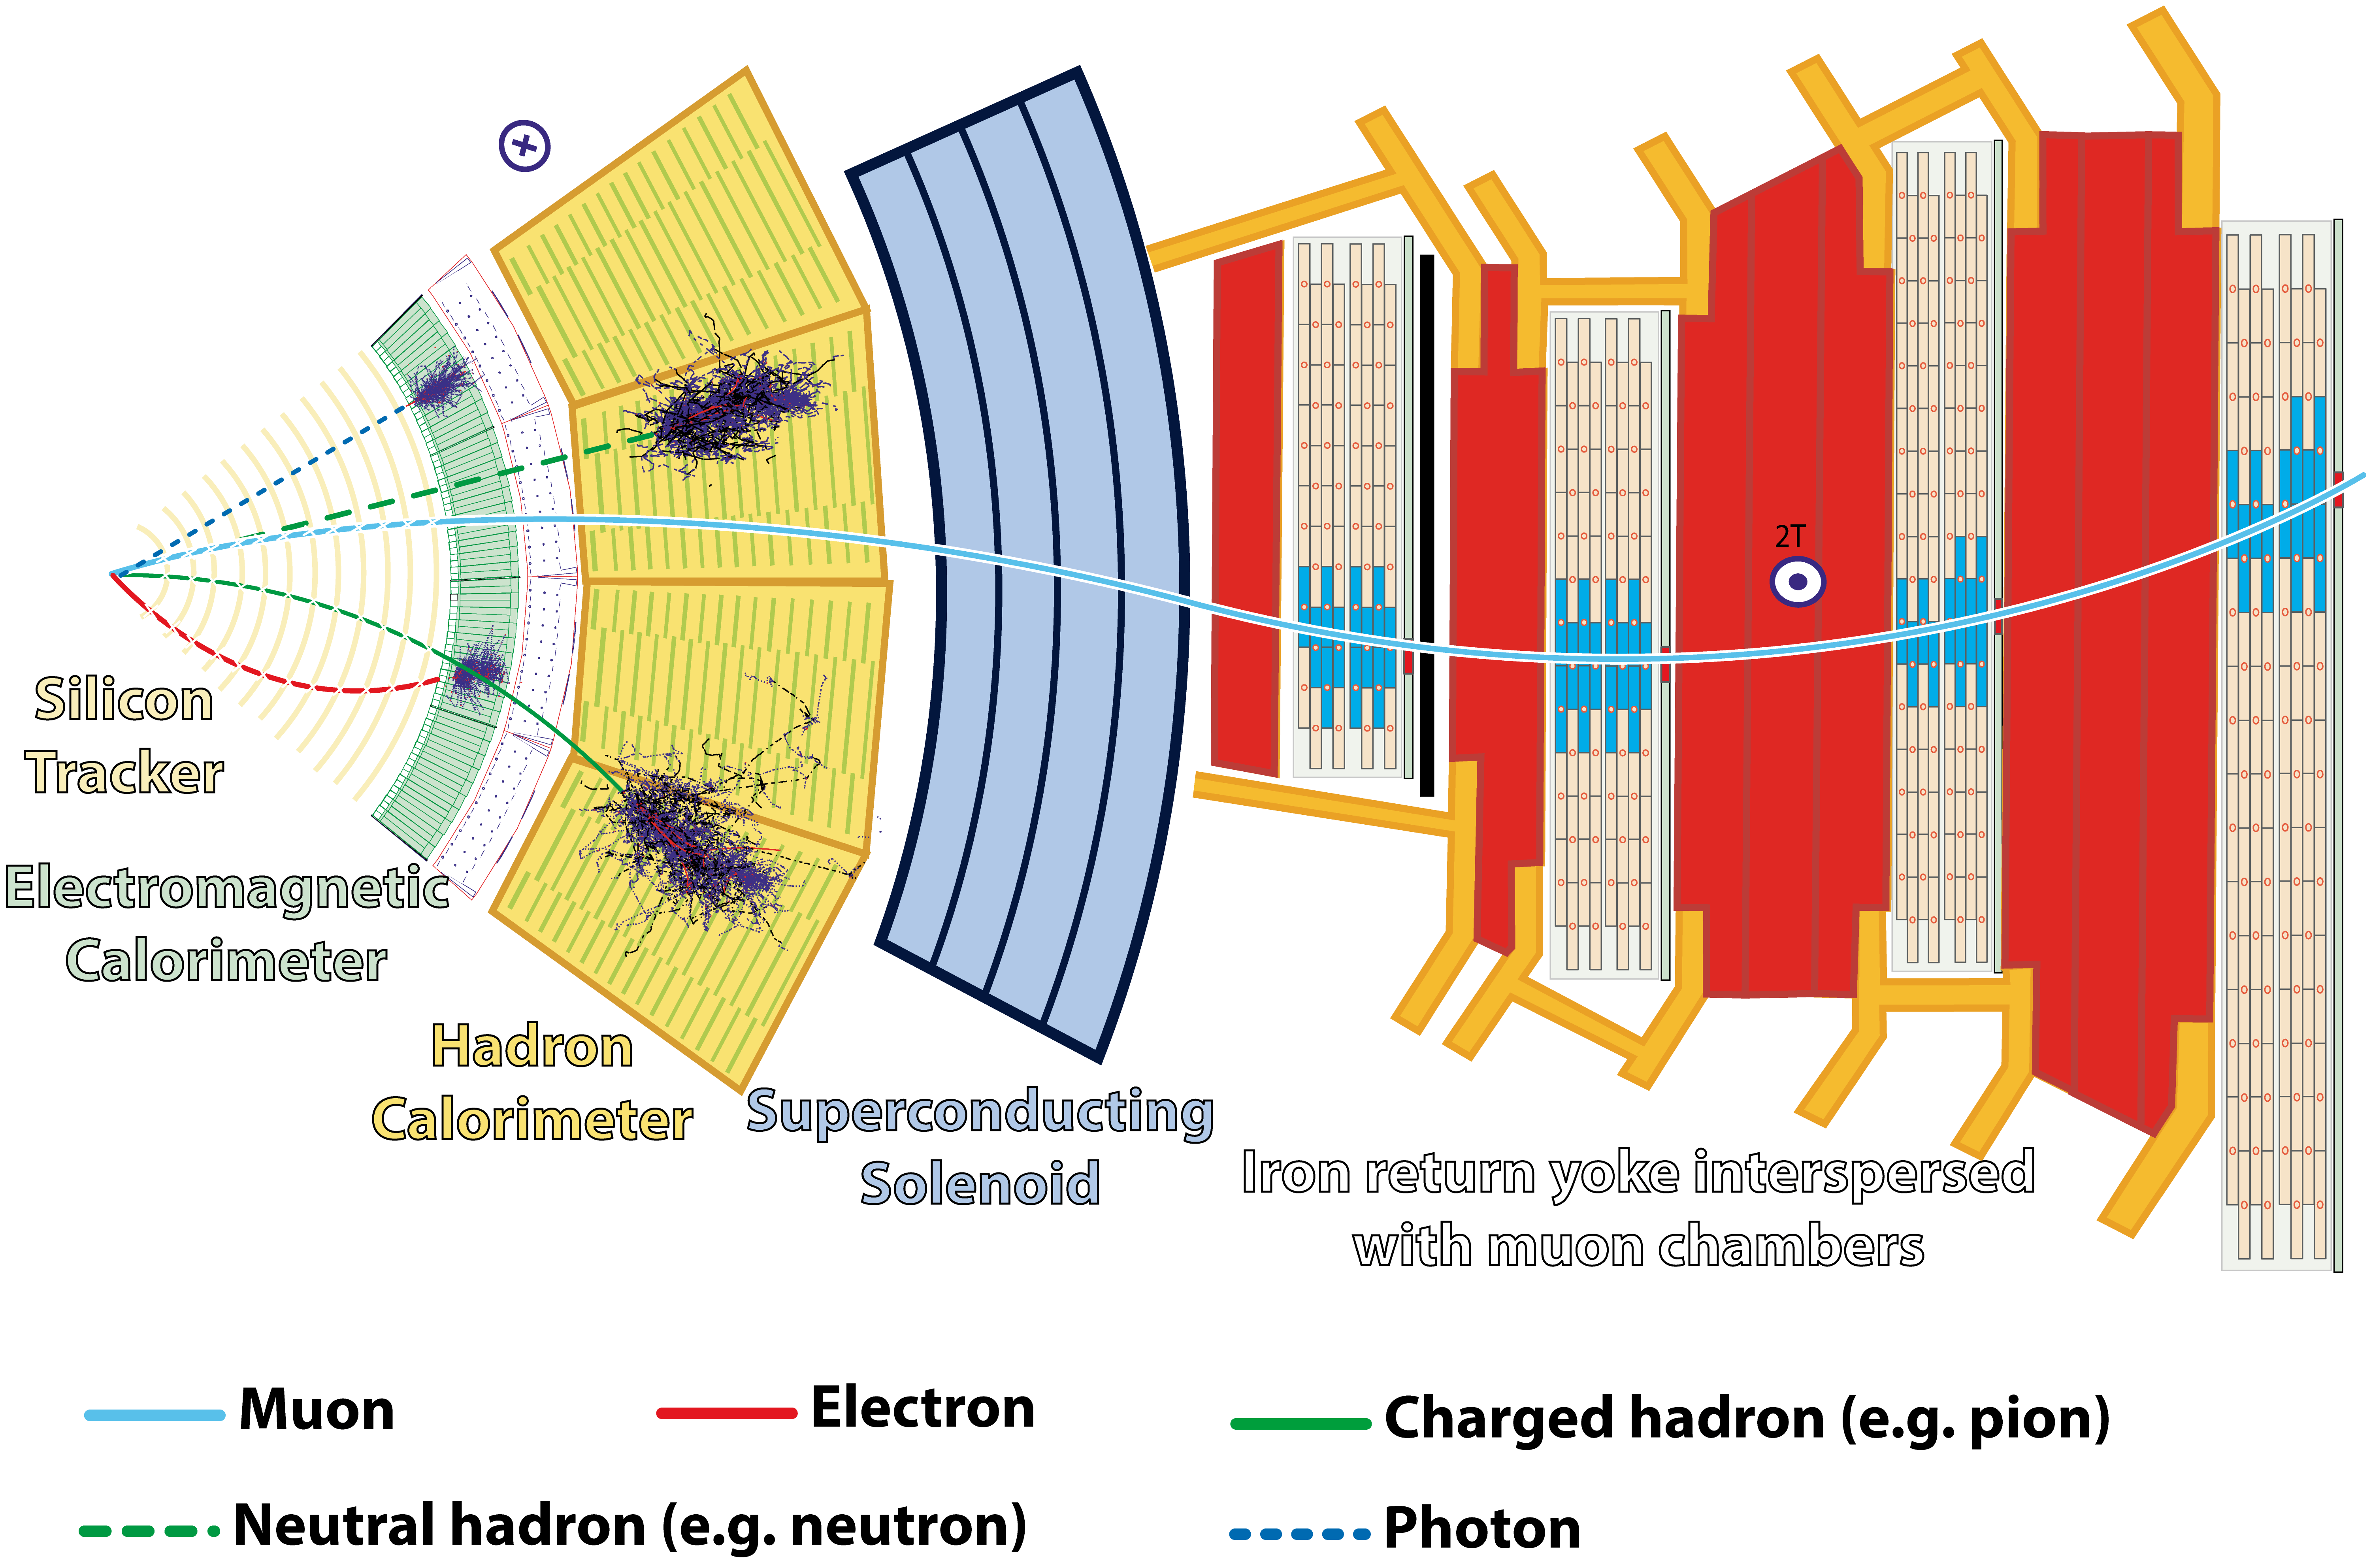
\includegraphics[width=0.5\linewidth]{CMSslice_whiteBackground (1).png}
    \caption{Caption}
    \label{fig:CMS_capas}
\end{figure}



\url{https://twiki.cern.ch/twiki/bin/view/CMSPublic/WorkBookCMSExperiment}


\chapter{Resultados y Análisis}
En todo el análisis se utilizarán unidades naturales...\\


Como ya se explicó en la introducción \textcolor{red}{EXPLICAR EN LA INTRODUCCIÓN} los eventos $t/\overline{t}$ + DM y $t\overline{t}$ + DM pueden contener cero, uno o dos leptones; referidos como eventos hadrónicos (AH, \textit{all hadronic}), semileptónicos (SL, \textit{single lepton}) o dileptónicos (DL, \textit{dilepton}). Este análisis se va a focalizar en los eventos $t/\overline{t}W$ + DM y $t\overline{t}$ + DM dileptónicos, centrándose en el decaimiento de dos bosones $W$ en pares electrón-neutrino o muón-neutrino. \\

A la hora de analizar los eventos es importante destacar cómo se simulan. Para ello se utiliza la herramienta de simulación de Montecarlo que permite modelar con gran precisión las colisiones protón-protón y las interaaciones que suceden en el interior del detector. En primer lugar, la generación de eventos consiste en modelar la colisión inicial y la producción de partículas a partir de las interacciones fundamentales descritas por la teoría cuántica de campos. Se utilizan herramientas como \texttt{PYTHIA} \cite{PYTHIA}, \texttt{POWHEG} \cite{POWHEG} o \texttt{MADGRAPH} \cite{MADGRAPH} . En esta etapa se incluyen fenómenos como la hadronización de los quarks y gluones, así como los decaimientos de partículas inestables según las probabilidades teóricas conocidas. Una vez los eventos son modelados, se simula cómo interactúan las partículas generadas con el detector. Para ello se utiliza \texttt{GEANT4} \cite{GEANT4}. Durante esta etapa se tienen en cuenta efectos como la pérdida de energía en los materiales, la dispersión múltiple y las respuestas de los sensores del detector, lo que permite obtener una simulación realista de los datos recolectados.\\


Durante el análisis se emplearán diversas variables leptónicas, sobre las cuales se podrán aplicar cortes para optimizar la búsqueda.


\begin{itemize}
    \item[\ding{220}] \texttt{events}: Número de eventos considerados en el análisis.

    \item[\ding{220}] \texttt{eta1} y \texttt{eta2}: Pseudorapidez del primer y segundo leptón. Se suele utilizar como coordenada espacial para indicar el ángulo con respecto al haz de partículas. 
    $$
    \eta = -\ln \left( \tan \left( \frac{\theta}{2}\right) \right)
    $$
    Donde $\theta$ es el ángulo entre el momento de la partícula $\vec{p}$ y el eje del haz.
    \item[\ding{220}] \texttt{dphill}: Diferencia en el ángulo azimutal de dos leptones.
    $$
    \Delta \phi_{ll} = |\phi_l^1-\phi_l^2|
    $$
    \item[\ding{220}] \texttt{dphillmet}: Diferencial en el ángulo azimutal entre la dirección de los leptones y la energía tranversa faltante.
    $$
    \Delta \phi_{ll,\text{MET}} = \phi_{ll}-\phi_\text{MET}
    $$
    \item[\ding{220}] \texttt{drll}: Distancia angular entre los dos leptones en el espacio $(\eta, \phi)$, definida como:
    $$
    \Delta R_{ll} = \sqrt{(\Delta \eta)^2+(\Delta \phi)^2}
    $$
    \item[\ding{220}] \texttt{mll}: Masa invariante del sistema dileptónico. Su ecuación es la siguiente:
    $$
    m_{\ell \ell} = \sqrt{(E_{\ell}^1 + E_\ell^2)^2-(\vec{p_\ell^1}+\vec{p_\ell^2})^2}
    $$
    Donde $E_\ell^i$ y $\vec{p}_\ell^i$ son la energía y el momento del leptón $i$-ésimo respectivamente.
    \item[\ding{220}] \texttt{mpmet}:  Magnitud del momento transverso faltante corregido, utilizado para mejorar la estimación de la energía faltante.
    $$
    E_T^{\text{miss}} = -\Bigg| \sum_i \vec{p_T^i} \Bigg|
    $$
    \item[\ding{220}] \texttt{puppimet}: Energía faltante calculada usando el algoritmo PUPPI, que mejora la resolución eliminando efectos del pileup.
    \item[\ding{220}] \texttt{pt1} y \texttt{pt2}: Momento del primer y segundo leptón en el eje transversal al eje del haz.
    $$
    p_T = \sqrt{p_x^2+p_y^2}
    $$
    \item[\ding{220}] \texttt{ptll}: Momento transverso del sistema dileptónico.
    $$
    p_T^{\ell \ell} = |\vec{p_T^{\ell 1}} + \vec{p_T^{\ell 2}}|
    $$
    \item[\ding{220}] \texttt{mth}: Masa transversa del sistema \textit{leading} leptón-MET, definida como:
    $$
    m_T^H = \sqrt{2p_T^{\ell 1}\cdot \text{MET}\cdot (1-\cos(\Delta \phi_{\ell 1, \text{MET}}))}
    $$
    \item[\ding{220}] \texttt{mtw2}: Masa transversal calculada considerando el segundo lepton y el MET, definida como:
    $$
    m_T^{W2} = \sqrt{2p_T^{\ell 2}\cdot \text{MET}\cdot (1-\cos(\Delta \phi_{\ell 2, \text{MET}}))}
    $$
    
    \item[\ding{220}] \texttt{mjj}: Masa invariante de dos \textit{jets} seleccionados:
    $$
    m_{j j} = \sqrt{(E_{j}^1 + E_j^2)^2-(\vec{p_j^1}+\vec{p_j^2})^2}
    $$
    Donde $E_j^i$ y $\vec{p}_j^i$ son la energía y el momento del \textit{jet} $i$-ésimo respectivamente.
\end{itemize}

Una vez definidas las variables relevantes para el análisis, es fundamental considerar los distintos procesos de fondo que pueden contribuir a los eventos observados. Estos fondos corresponden a eventos del Modelo Estándar que imitan la firma esperada de la señal y pueden dificultar su identificación.

\begin{itemize}
    \item[\ding{220}] $t\overline{t}$: Eventos de producción de un par top-antitop que decaen en dos leptones y dos neutrinos. Es decir, los quarks top decaen de la forma : $t \rightarrow W^+b$, $\overline{t} \rightarrow W^-\overline{b}$ y los bosones W decaen como $W^+ \rightarrow l^+\nu$, $W^- \rightarrow l^-\overline{\nu}$.

    \item[\ding{220}] Single top: Se refiere a la producción de un único quark top (o antitop)  en vez de un par $t\overline{t}$. Se puede dar principalmente a través de tres canales: \textit{s-channel} donde un bosón $W$ virtual decae en un par $t\overline{b}$, \textit{t-channel} donde un bosón $W$  virtual se intercambia entre un par $qb$ y $q't$ y la producción de un par $tW$ a partir de un par $gb$. \cite{SingleTop}

    \item[\ding{220}] Semi Leptonic: Este fondo se refiere a eventos $t\overline{t}$ donde uno de los quarks decae hadrónicamente y otro decae leptónicamente.

    \item[\ding{220}] $tt$V: Categoría donde se engloban los eventos con producción de un par top-antitop con un bosón $Z$, $W$ o Higgs. Se tiene en cuenta además las diferentes maneras que tiene cada bosón en decaer. Esto es, el bosón $Z$ puede decaer en 2 leptones o 2 neutrinos o puede hadronizar. El bosón $W$ puede decaer en un par leptón-neutrino o puede hadronizar.  Los eventos con Higgs pueden decaer de la siguiente manera: $t\overline{t}H \rightarrow (W^+b)(W^-\overline{b})(b\overline{b})$ y decayendo el par $t\overline{t}$ decaen por el canal dileptónico o pueden no decaer en un par $b\overline{b}$ sino en otros modos. \cite{ttV}
    
 \item[\ding{220}] VV: Producción de un par de bosones vectoriales ($W^+W^-, W^\pm Z, ZZ$). Se tienen en cuenta cuando el par de bosones $W$ decae de manera dileptónica. El par $W^\pm Z$ puede decaer en 3 leptones y un neutrino, 2 leptones y en quarks (hadronización). Por último, el par $ZZ$  puede decaer en 2 leptones y 2 neutrinos, se puede hadronizar y decaer en quarks y 2 leptones o en 4 leptones.

 \item[\ding{220}] Drell-Yan (DY): El proceso de Drell-Yan ocurre cuando se aniquila un quark-antiquark en colisiones hadrónicas, creando un bosón $Z$ o un fotón virtual que decaen en un par de leptones con carga opuesta. \cite{wiki:Drell–Yan_process}

 \item[\ding{220}] \textit{Other}: En esta categoría se incluyen eventos que pueden ser de interés pero que no se corresponden a ningún otro grupo de eventos. Por ejemplo, pares $Z\gamma$ que decaen en 2 leptones y un fotón o eventos con Higgs.
\end{itemize}


\section{Adaptación del análisis}

El \textit{framework} del trabajo estaba inicialmente orientado a la búsqueda de señales de WW + DM en los datos, con selección y cortes optimizados para ese canal. \cite{CMSWW} Sin embargo, el enfoque se ha modificado para centrarse en la búsqueda de firmas de producción de pares de quarks top-antitop. Esto ha implicado ajustes en los criterios de selección de eventos, en la definición de regiones de señal y fondo, y en la estrategia general del análisis para maximizar la sensibilidad a esta nueva hipótesis. Mientras que en la búsqueda de  WW+DM se priorizaban eventos con estados finales leptónicos y MET significativo, el análisis de $t\overline{t}$ requiere una identificación precisa de b-jets y una reconstrucción más detallada de los decaimientos hadrónicos, semileptónicos o dileptónicos de los quarks top.\\

Durante todo el análisis se va a utilizar un modelo teórico de materia oscura simplificada. Se asumen que las partículas de materia oscura $\chi$ son fermiones y los mediadores $\phi$ son partículas con \textit{spin} 0. Las constantes de acoplamiento tanto entre el mediador y las partículas del modelo estándar $g_q$ como entre las partículas mediadoras con las partículas fermiónicas de materia oscura $g_\chi$ se asume por simplicidad $g_q = g_\chi = 1$. Los dos parámetros que quedan libres son las masas de las partículas $\chi$ y $\phi$. Se van a definir 17 puntos de masa distintos: variando la masa de la partícula mediadora entre 50 a 500 GeV en pasos de 50 GeV dejando fija la masa de la partícula de materia oscura a $m_\chi = 1$ GeV y fijando la masa del mediador $m_\phi = 100$ GeV y variando la masa del fermión $m_\chi = \{ 20, 30 ,40 ,45, 49 ,51, 55 \}$ GeV. De ahora en adelante, los puntos de masa se representarán con dos números en un paréntesis separados con un símbolo de coma, de manera que ($m_\chi$, $m_\phi$).\\

En la figura \ref{fig:comparacion_analisisWW_tt} se puede observar un \textit{stack plot} donde se ve la diferencia entre nuestro análisis y en el que nos hemos inspirado. Los \textit{stack plots} son un tipo de gráficas que se suele utilizar en la rama de la física de partículas donde se muestra las diferentes contribuciones a una distribución de manera que los fondos aparecen apilados unos sobre otros. En el eje x aparece la variable que se estudia (en este caso, la masa invariante) dividida en pequeños intervalos llamados \textit{bins}. Cada proceso físico ($t\overline{t}$, DY, $tt$V...) se representa con un histograma de distinto color, de manera que la altura total de cada \textit{bin} representa el número total de eventos esperados. Las señales se muestran con líneas sin apilar. Aparte de los histogramas apilados aparecen puntos de datos experimentales para comparar la diferencia entre los eventos simulados y los eventos reales, también llamado \textit{mismodelling}. En este caso se representa la masa invariante de los leptones en ambos casos. Se puede observar el cambio en los eventos a analizar y que se pinta en la gráfica dos regiones de señal: en azul cían para la producción de partículas de materia oscura con masa (1, 50) y en naranja para partículas con masa (1, 500).
 

\begin{figure}[h!]
     \centering
     \begin{subfigure}[b]{0.43\textwidth}
         \centering
         \includegraphics[width=\textwidth]{images/log_cratio_dhww2l2v_13TeV_sr_1bj_mll_ANALISISWW.png}
         \caption{Signatura $WW$ + DM}
         \label{fig: ANALISISWW}
     \end{subfigure}
     \begin{subfigure}[b]{0.43\textwidth}
         \centering
         \includegraphics[width=\textwidth]{images/log_cratio_dhww2l2v_13TeV_sr_emu_1bj_mll.png}
         \caption{Signatura $t\overline{t}$ + DM}
         \label{fig: ANALISISttbar}
     \end{subfigure}
     \hfill
     \caption{Comparación entre las categorías del análisis con signatura $WW$ + DM  y las categorías del análisis con signatura $t\overline{t}$ + DM.}
     \label{fig:comparacion_analisisWW_tt}

\end{figure}



\section{Selección de sucesos básica}

Uno de los objetivos del trabajo es intentar maximizar la señal que queremos observar frente al fondo total. Para ello se aplican cortes y selecciones en las distintas variables y se impone tener en cuenta ciertos eventos. Todo el análisis va a estar inspirado en el \textcolor{cyan}{Analysis Note}. A partir de ahora se considerarán los eventos $t/\overline{t}$ + DM y $t\overline{t
}$ que contengan dos leptones (canal DL).\\

El análisis se lleva a cabo en un principio en tres canales distintos: canal electrón-electrón $ee$, canal electrón-muón $e\mu$ y canal muón-muón $\mu \mu$. Para esta selección se impone que los dos leptones que se generan tengan carga opuesta y se excluyen eventos unileptónicos. También se fuerza que el $p_T$ del leptón \textit{leading} (el que tiene el mayor $p_T$) sea mayor que 25 GeV y el leptón \textit{trailing} (el que tiene el segundo mayor $p_T$) sea mayor que 20 GeV. Esto se hace para que no se tenga en cuenta las regiones con $p_T$ pequeñas ya que así se reduce contribuciones al fondo y se excluyen zonas de baja eficiencia del detector. Además, si hay 3 leptones se excluyen los eventos cuyo $p_T$ del tercer leptón sea mayor de 10 GeV. Así se evitan eventos donde haya 3 o más leptones significativos. Se impone además un corte en $m_{ll}$, que tiene que ser mayor que 20 GeV para evitar resonancias a bajas energías. Para que se reduzca aún más el fondo DY, en los canales $ee$ y $e\mu$ se aplica un veto en $m_{ll}$ alrededor de la masa del bosón Z. Finalmente se aplica un corte a mpmet y puppimet para...........\\

Dentro de estas preselecciones se crean diferentes categorías atendiendo al número de jets que se crean a partir de la hadronización de un quark bottom (b-jets). La condición para que un jet se considere b-jet es que su momento transverso sea mayor de 30 GeV, debe tener una pseudorapidez de $|\eta| < 2.5$ y un valor del discriminante de b-jets (una manera de indicar cómo de probable es de confundir un jet por un b-jet) de 0.1241, correspondiente a un \textit{Medium Working Point}. \cite{LooseWorkingPoint} Para cada par leptónico ($ee$, $e\mu$,  $\mu\mu$) y dependiendo cuantos b-jets se han reconocido se han definido 5 categorías: la categoría \textbf{in} no impone ninguna condición sobre el número de b-jets, \textbf{0bj} cuando no se ha reconocido ningún b-jet, \textbf{eq1bj} cuando se ha reconocido exactamente 1, \textbf{1bj} cuando se ha reconocido 1 o más y \textbf{2bj} cuando se ha reconocido 2 o más. Como se puede esperar, la categoría \textbf{in} es la más inclusiva. 

\begin{table}[h!]
\centering
\begin{tabular}{|ccccc|}
\hline
\multicolumn{5}{|c|}{\textbf{Selección básica}}                                                                               \\ \hline

\multicolumn{1}{|c|}{\textbf{in}} & \multicolumn{1}{c|}{\textbf{0bj}}          & \multicolumn{1}{c|}{\textbf{1bj}}            & \multicolumn{1}{c|}{\textbf{eq1bj}}        & \multicolumn{1}{c|}{\textbf{2bj}}          \\ \hline

\multicolumn{1}{|c|}{$n_{bJ} \ge 0$} & \multicolumn{1}{c|}{$n_{bJ} = 0$} & \multicolumn{1}{c|}{$n_{bJ} \ge 1$} & \multicolumn{1}{c|}{$n_{bJ} = 1$} & \multicolumn{1}{c|}{$n_{bJ} \ge 2$}    \\ \hline
\multicolumn{5}{|c|}{$q_{l1} \cdot q_{l2} < 0$}                                                                                 \\ \hline
\multicolumn{5}{|c|}{$n_l \ge 2$}                                                                                             \\ \hline
\multicolumn{5}{|c|}{$p_T^{l1} > 25 $ GeV}                                                                                       \\ \hline
\multicolumn{5}{|c|}{$p_T^{l2} > 20 $ GeV}                                                                                       \\ \hline
\multicolumn{5}{|c|}{Si $n_l > 2$, $p_T^{l3} < 10$ GeV}                                                                          \\ \hline
\multicolumn{5}{|c|}{$m_{ll}> 20$ GeV, si el sabor del leptón es el mismo: $|m_{ll}-m_Z| > 15 $ GeV}                           \\ \hline
\multicolumn{5}{|c|}{mpmet $> 20$ GeV}                                                                                        \\ \hline
\multicolumn{5}{|c|}{PUPPImet $>$ 20 GeV}                                                                                     \\ \hline

\end{tabular}
\caption{\textcolor{cyan}{Cambiar el formato}}
\label{tab:preseleccion_basica}
\end{table} 



En la figura \ref{fig:comparacion_preseleccion_basica} se muestran los \textit{stack plots} de la $m_{\ell \ell}$ y $p_T^{\ell \ell}$ para alguna de las regiones de esta selección. Se puede observar en las gráficas correspondientes a $m_{\ell \ell}$ los cortes en la región del bosón Z. También se puede destacar cómo en las categorías $ee$ y $\mu \mu$ el fondo de Drell-Yan es más importante que en el caso de $e \mu$, debido a producciones de pares leptónicos del mismo sabor por fotones virtuales o por la resonancia del bosón Z.\\


\begin{figure}[h!]
     \centering
     \begin{subfigure}[b]{0.32\textwidth}
         \centering
         \includegraphics[width=\textwidth]{images/log_cratio_dhww2l2v_13TeV_sr_ee_1bj_mll.png}
         \caption{Categoría $ee$\_in}
         \label{fig: ANALISISWW}
     \end{subfigure}
     \begin{subfigure}[b]{0.32\textwidth}
         \centering
         \includegraphics[width=\textwidth]{images/log_cratio_dhww2l2v_13TeV_sr_mumu_1bj_mll.png}
         \caption{Categoría $\mu \mu$\_in}
         \label{fig: ANALISISttbar}
     \end{subfigure}
     \begin{subfigure}[b]{0.32\textwidth}
         \centering
         \includegraphics[width = \textwidth]{images/log_cratio_dhww2l2v_13TeV_sr_emu_1bj_mll.png}
         \caption{Categoría $e \mu$\_in}
         \label{}
     \end{subfigure}
     \hfill
    \begin{subfigure}[b]{0.32\textwidth}
        \centering
         \includegraphics[width = \textwidth]{images/log_cratio_dhww2l2v_13TeV_sr_ee_ptll.png}
         \caption{Categoría $e \mu$\_in}
         \label{}
     \end{subfigure}
         \begin{subfigure}[b]{0.32\textwidth}
        \centering
         \includegraphics[width = \textwidth]{images/log_cratio_dhww2l2v_13TeV_sr_mumu_ptll.png}
         \caption{Categoría $e \mu$\_in}
         \label{}
     \end{subfigure}
         \begin{subfigure}[b]{0.32\textwidth}
        \centering
         \includegraphics[width = \textwidth]{images/log_cratio_dhww2l2v_13TeV_sr_emu_ptll.png}
         \caption{Categoría $e \mu$\_in}
         \label{}
     \end{subfigure}
     
     \caption{Histogramas obtenidos para la selección básica. En la fila de arriba se representan las gráficas para la variable $m_{\ell \ell}$ y en la fila de abajo para la variable $p_T^{\ell \ell}$.}     \label{fig:comparacion_preseleccion_basica}

\end{figure}

Durante el análisis se ha visto que para las categorías $ee$ y $\mu\mu$ el \textit{mismodelling} para energía transversa perdida era bastante significativo, esto puede ser debido a inconsistencias en la determinación de los fondos con un leptón genuino y uno instrumental. Con el fin de sacar mejores conclusiones en el estudio, a partir de ahora solo se tendrán en cuenta los eventos de la categoría $e \mu$.\\


\section{Selección del análisis}

Para la selección del análisis se va a utilizar únicamente eventos que ocurran en el canal $e\mu$ cuyas cargas sean opuestas. Se van a definir tres regiones atendiendo al número de b-jets: $t/\overline{t}$ + DM para eventos con un único b-jet, $t\overline{t}$ + DM para eventos con 2 o más b-jets y $tt\overline{t}$ + DM para el caso más inclusivo donde hay 1 o más b-jets.  A continuación se imponen ciertos cortes en los momentos transversos para los leptones \textit{leading} y \textit{trailing} para que sean mayor que 25 GeV y 20 GeV respectivamente. Además, se pide que el número de leptones sea exactamente igual a 2. Por último se toman los eventos cuyo $m_{ll}$ sea mayor que 20 GeV y los eventos donde al menos haya un jet.\newpage

\begin{table}[h!]
\centering
\begin{tabular}{|ccc|}
\hline
\multicolumn{3}{|c|}{\textbf{Selección del análisis}}                                                  \\ \hline
\multicolumn{1}{|c|}{$t$\textbf{DM}} & \multicolumn{1}{c|}{$tt$\textbf{DM}} & \textbf{$tt\overline{t}$DM} \\ \hline
\multicolumn{1}{|c|}{$n_{bJ} = 1$}       & \multicolumn{1}{c|}{$n_{bJ} \ge 2$}    & $n_{bJ} \ge 1$     \\ \hline
\multicolumn{3}{|c|}{Canal $e\mu$, $q_{l1} \cdot q_{l2} < 0$}                                            \\ \hline
\multicolumn{3}{|c|}{$n_l = 2$}                                                                        \\ \hline
\multicolumn{3}{|c|}{$n_J \ge 1$} 
                        \\ \hline
\multicolumn{3}{|c|}{$p_T^{l1} > 25 $ GeV}                                                                \\ \hline
\multicolumn{3}{|c|}{$p_T^{l2} > 20 $ GeV}                                                                \\ \hline
\multicolumn{3}{|c|}{Si $n_l > 2$, $p_T^3 < 10$ GeV}                                                   \\ \hline
\multicolumn{3}{|c|}{$m_{ll}> 20$ GeV}                                                                 \\ \hline

\end{tabular}
\caption{Selección básica aplicada a los procesos del análisis.}
\label{tab:preseleccion_anlisis}
\end{table}

En la figura \ref{fig:Stack_PreseleccionAN} se muestran los histogramas para algunas variables de esta selección. En este caso no se va a hacer hincapié en los datos experimentales y por tanto se representa unicamente la simulación.\newpage
\begin{figure}[h!]
     \centering
     \begin{subfigure}[b]{0.43\textwidth}
         \centering
         \includegraphics[width=\textwidth]{images/log_cratio_dhww2l2v_13TeV_sr_emu_tttDM_ptll.png}
         \caption{Variable \texttt{ptll}}
         \label{fig:stack_tttDM_ptll}
     \end{subfigure}
     \begin{subfigure}[b]{0.43\textwidth}
         \centering
         \includegraphics[width=\textwidth]{images/log_cratio_dhww2l2v_13TeV_sr_emu_tttDM_mll.png}
         \caption{Variable \texttt{mll}}
         \label{fig:stack_tttDM_mll}
     \end{subfigure}
     \hfill
          \begin{subfigure}[b]{0.43\textwidth}
         \centering
         \includegraphics[width=\textwidth]{images/log_cratio_dhww2l2v_13TeV_sr_emu_tttDM_mpmet.png}
         \caption{Variable \texttt{mpmet}}
         \label{fig:stack_tttDM_mpmet}
     \end{subfigure}
          \begin{subfigure}[b]{0.43\textwidth}
         \centering
         \includegraphics[width=\textwidth]{images/log_cratio_dhww2l2v_13TeV_sr_emu_tttDM_mtw2.png}
         \caption{Variable \texttt{mtw2}}
         \label{fig:stack_tttDM_mtw2}
     \end{subfigure}
     \caption{\textcolor{red}{VARIABLE MPMET TIENE 'DOS SEÑALES'} Histogramas para algunas variables de la categoría tttDM del análisis. }
     \label{fig:Stack_PreseleccionAN}
\end{figure}

Se puede observar que en las variables \texttt{mpmet} y \texttt{mtw2} el comportamiento de fondo y señal difieren mucho. Esto nos sugiere sobre qué variable centrarnos en buscar cortes óptimos.

\section{Optimización de la señal y automatización}

Con el fin de optimizar los cortes para maximizar la sensibilidad a la señal que se busca se estudiará la figura de mérito (FOM, por sus siglas en inglés \textit{Figure of Merit}) de las distintas distribuciones. Este procedimiento es muy recurrente en el contexto de la física de partículas, ya que minimiza la contribución del fondo en nuestro análisis. La figura de mérito tiene la siguiente expresión:

\begin{equation}\label{eq: fom}
    \text{FOM} = \frac{S}{\sqrt{S+B}}
\end{equation}

Donde $S$ son los sucesos de señal y $B$ son los sucesos de fondo. La idea de este apartado es calcular la figura de mérito en dos variables: \texttt{mpmet} y \texttt{mtw2}. Se iterará para cada \textit{bin} y se encontrará el valor de la variable que maximiza la figura de mérito. Estos valores serán los cortes óptimos para mpmet y mtw2.\\


Se ha creado dos códigos para el cálculo de la figura de mérito, que se exponen en el Apéndice \textcolor{cyan}{NÚMERO}, llamados \texttt{1D$\_$opti$\_$fom.py} y \texttt{2D$\_$opti$\_$fom.py}. En nuestro análisis nos va a interesar optimizar 2 variables: \texttt{mpmet} y \texttt{mtw2}. La diferencia entre ambos códigos es que el primero se utiliza para optimizar únicamente una de las dos variables, mientras que el segundo código se utiliza para optimizar las dos a la vez con el objetivo de ahorrar un poco de tiempo. Se ha tomado como eventos de señal las correspondientes a la creación de partículas de materia oscura para diferentes puntos de masa. \\

El algoritmo para el cálculo de la figura de mérito se presenta a continuación. Inicialmente se definen los argumentos que se pasarán por terminal a la hora de correr el código. El código abre el archivo de \texttt{ROOT} que contiene los histogramas y recorre todos los directorios correspondientes a las distintas categorías. Una vez localizada la categoría que se quiere estudiar, se accede al directorio correspondiente y se recorren todos los \textit{bins} que componen los histogramas. Si el nombre del histograma es el mismo que el de la región de señal, se almacena en la variable \texttt{SIGNAL} el valor de la integral del histograma. La integral puede calcularse de dos maneras: acumulando desde el $bin$ inicial hasta el $bin$ actual (integral desde la izquierda) o desde el $bin$ actual hasta el $bin$ final (integral desde la derecha). Si el nombre del histograma no coincide con el de la señal, el valor de la integral se le suma a la variable \texttt{TOTAL}. Tras esto, se calcula el valor de la figura de mérito según la ecuación \ref{eq: fom} y se comprueba si es su valor máximo hasta ese momento. En caso afirmativo, se almacena el valor máximo de la FOM junto con el corte óptimo, la cantidad de eventos de señal y de fondo. El código además tiene un par de funciones para crear las gráficas de la figura de mérito y los \textit{shapes plots}.\\

Inicialmente se ha calculado la figura de mérito para las dos variables de manera independiente, obteniendo los siguientes resultados:\\

\begin{figure}[h!]
     \centering
     \begin{subfigure}[b]{0.43\textwidth}
         \centering
         \includegraphics[width=\textwidth]{images/emu__tttDM_FOM_mpmet_mchi1_mphi100.png}
         \caption{Variable mpmet}
         \label{fig: ANALISISWW}
     \end{subfigure}
     \begin{subfigure}[b]{0.43\textwidth}
         \centering
         \includegraphics[width=\textwidth]{images/emu__tttDM_FOM_mtw2_mchi1_mphi100.png}
         \caption{Variable mtw2}
         \label{fig: ANALISISttbar}
     \end{subfigure}
     \hfill
     \caption{Gráficas de la figura de mérito para las dos variables a analizar en la categoría \_tttDM y punto de masa (1, 100).}
     \label{fig:FOM_sincortes_mpmet_mtw2}
\end{figure}

En la tabla \ref{tab:fom_binxbin_tttDM_1_100} se refleja el análisis de la figura de mérito realizado sobre la muestra punto de masa es (1, 100) para la variable \texttt{mpmet} y categoría $\_$tttDM. Se ve que el valor de \texttt{mpmet} que mejor caracteriza la señal es \texttt{mpmet} = 110 GeV.  



\begin{table}[h!]
\centering
\begin{tabular}{ |c|c|c|c|c| }
 \hline
Corte del \textit{bin} [GeV]  & S (Señal) &  Fondo(S+B)  & FoM &  Corte óptimo [GeV] \\    \hline
0.00 & 2291.99 & 351298.18 & 3.87 & 0.00 \\
 \hline
10.00 & 2050.47 & 317032.83 & 3.64 & 0.00 \\
 \hline
20.00 & 1864.42 & 283576.66 & 3.50 & 0.00 \\
 \hline
30.00 & 1705.47 & 240643.33 & 3.48 & 0.00 \\
 \hline
40.00 & 1557.08 & 197946.38 & 3.50 & 0.00 \\
 \hline
50.00 & 1414.15 & 156504.48 & 3.57 & 0.00 \\
 \hline
60.00 & 1275.58 & 118180.96 & 3.71 & 0.00 \\
 \hline
70.00 & 1140.85 & 85151.33 & 3.91 & 70.00 \\
 \hline
80.00 & 1015.29 & 59087.08 & 4.18 & 80.00 \\
 \hline
90.00  & 892.22 & 40406.31 & 4.44 & 90.00 \\
 \hline
100.00 & 778.15 & 28039.25 & 4.65 & 100.00 \\
 \hline
110.00 & 675.75 & 20182.67 & 4.76 & 110.00 \\
 \hline
120.00 & 581.77 & 15238.73 & 4.71 & 110.00 \\
 \hline
130.00 & 499.01 & 11999.99 & 4.56 & 110.00 \\
 \hline
140.00 & 426.76 & 9750.00 & 4.32 & 110.00 \\
 \hline
150.00 & 364.28 & 8102.34 & 4.05 & 110.00 \\
 \hline
160.00 & 307.57 & 6823.53 & 3.72 & 110.00 \\
 \hline
170.00 & 260.32 & 5790.59 & 3.42 & 110.00 \\
 \hline
180.00 & 220.83 & 4942.90 & 3.14 & 110.00 \\
 \hline
190.00 & 187.40 & 4234.90 & 2.88 & 110.00 \\
 \hline
200.00 & 158.79 & 3632.04 & 2.63 & 110.00 \\
 \hline
210.00 & 133.18 & 3121.74 & 2.38  & 110.00 \\
 \hline
220.00 & 112.93 & 2677.86 & 2.18 & 110.00 \\
 \hline
230.00 & 94.43 & 2303.46 & 1.97 & 110.00 \\
 \hline
240.00 & 80.83 & 1993.71 & 1.81 & 110.00 \\
 \hline
250.00 & 68.11 & 1713.72 & 1.65 & 110.00 \\
 \hline
260.00 & 57.90 & 1483.86 & 1.50 & 110.00 \\
 \hline
270.00 & 48.70 & 1281.27 & 1.36 & 110.00 \\
 \hline
280.00 & 42.24 & 1107.54 & 1.27 & 110.00 \\
 \hline
290.00 & 36.65 & 960.57 & 1.18 & 110.00 \\
 \hline

\end{tabular}
\caption{Valor del corte del \textit{bin}, el número de eventos de señal $S$, el número total de eventos del fondo $S+B$, el valor de la figura de mérito según la ecuación \ref{eq: fom} y el valor del corte óptimo hasta el \textit{bin} correspondiente.}
\label{tab:fom_binxbin_tttDM_1_100}
\end{table}


Como se puede ver, la figura de mérito tiene su máximo alrededor de 110 GeV para la variable mpmet y \textcolor{red}{120} GeV para la variable mtw2. Se utilizarán estos valores como cortes óptimos ya que maximizan la sensibilidad de la señal.\\


Como se tienen 17 regiones de señal, sería conveniente realizar esto para todas ellas. Mediante el uso de un nuevo archivo \texttt{opti\_all.sh} se ha iterado la búsqueda de los cortes óptimos en las 2 variables \texttt{mpmet} y \texttt{mtw2} para todos los puntos de masa. A continuación se muestra una tabla con los cortes óptimos para todos los puntos de masa, junto a los eventos de señal y fondo y el valor de la figura de mérito.
\newpage

\begin{table}[h!]
\centering
\begin{tabular}{ |c| |c| |c| |c| |c| }
 \hline
Punto de masa [GeV] & Corte óptimo [GeV] & Señal(S) & Fondo(S+B) & FoM \\
 \hline
(1, 50) & 110.00 & 570.79 & 20182.67 & 4.02 \\
 \hline
(1, 100) & 110.00 & 675.75 & 20182.67 & 4.76 \\
 \hline
(1, 150) & 120.00 & 640.76 & 15238.73 & 5.19 \\
 \hline
(1, 200) & 120.00 & 639.39 & 15238.73 & 5.18 \\
 \hline
(1, 250) & 120.00 & 695.62 & 15238.73 & 5.64 \\
 \hline
(1, 300) & 130.00 & 649.03 & 11999.99 & 5.92 \\
 \hline
(1, 350) & 130.00 & 660.75 & 11999.99 & 6.03 \\
 \hline
(1, 400) & 130.00 & 676.99 & 11999.99 & 6.18 \\
 \hline
(1, 450) & 130.00 & 702.39 & 11999.99 & 6.41 \\
 \hline
(1, 500) & 130.00 & 708.54 & 11999.99 & 6.47 \\
 \hline
(20, 100) & 110.00 & 677.82 & 20182.67 & 4.77 \\
 \hline
(30, 100) & 110.00 & 675.32 & 20182.67 & 4.75 \\
 \hline
(40, 100) & 110.00 & 678.00 & 20182.67 & 4.77 \\
 \hline
(45, 100) & 110.00 & 678.35 & 20182.67 & 4.77 \\
 \hline
(49, 100) & 120.00 & 575.90 & 15238.73 & 4.67 \\
 \hline
(51, 100) & 120.00 & 609.80 & 15238.73 & 4.94 \\
 \hline
(55, 100) & 120.00 & 650.36 & 15238.73 & 5.27 \\
 \hline

\end{tabular}
\caption{Cortes óptimos para cada punto de masa con su correspondientes eventos de señal, fondo y figura de mérito para la variable \texttt{mpmet} en la categoría tttDM.}
\label{tab:auto}
\end{table}

Otra manera de analizar los datos es utilizar un \textit{shape plot} en vez de un \textit{stack plot}. Los \textit{shape plots} son gráficos donde se muestra la forma normalizada de una distribución en vez de mostrar el número absoluto de eventos. Esto se realiza con el fin de evaluar la discriminación entre fondo y señal y comparar la forma de la distribución en diferentes regiones. Al igual que en los \textit{stack plots}, en el eje x se muestra la variable a analizar. Sin embargo, en el eje y aparecen la frecuencia normalizada de los eventos de señal y de fondo. Esto se realiza, al igual que con la figura de mérito, para los eventos de señal y fondo de las variables \texttt{mpmet} y \texttt{mtw2} los distintos puntos de masa.\\

\begin{figure}[h!]
     \centering
     \begin{subfigure}[b]{0.43\textwidth}
         \centering
        \includegraphics[width=\textwidth]{images/Shapes_mpmet__tttDM_mchi1_mphi100.png}
         \caption{Variable \texttt{mpmet}}
         \label{fig: Shapes_signal_bckg_mpmet}
     \end{subfigure}
     \begin{subfigure}[b]{0.43\textwidth}
         \centering
         \includegraphics[width=\textwidth]{images/Shapes_mtw2__tttDM_mchi1_mphi100.png}
         \caption{Variable \texttt{mtw2}}
         \label{fig: Shapes_signal_bckg_mtw2}
     \end{subfigure}
     \hfill
     \caption{\textit{Shape plots} para las dos variables \texttt{mpmet} y \texttt{mtw2} para el punto de masa (1, 100) en la categoría \_tttDM. En azul se refleja los eventos (normalizados) del fondo mientras que en rojo se muestra los eventos de señal.}
     \label{fig:Shapes_signal_bckg}
\end{figure}

Se puede ver claramente varias regiones diferenciadas. Si nos fijamos, por ejemplo, en la figura \ref{fig: Shapes_signal_bckg_mtw2} se ve como en la región de bajos valores hay una gran contaminación del fondo, por lo que no es ideal para la selección de eventos de señal. Alrededor de 120 GeV el número de eventos de señal y de fondo se comienza a igualar, y en valores grande la señal comienza a dominar. Esto sugiere dónde realizar el corte para mejorar la selección de señal.\\


Para evaluar el rendimiento de dos variables, se calculó la integral de la figura de mérito  en dos regiones distintas: la región donde predomina el fondo (FOM$_\text{f}$) y la región donde predomina la señal (FOM$_\text{s}$). Las regiones se dividieron en los rangos de 80 GeV y 110 GeV para \texttt{mpmet} y \texttt{mtw2} respectivamente.

Los resultados obtenidos fueron los siguientes:

\begin{itemize}
    \item Para la variable \texttt{mpmet}:
        \begin{itemize}
            \item FOM$_\text{f}$ = 33.37
            \item FOM$_\text{s}$ = 62.63
        \end{itemize}
    \item Para la variable \texttt{mtw2}:
        \begin{itemize}
            \item FOM$_\text{f}$ = 43.42
            \item FOM$_\text{s}$ = 45.17
        \end{itemize}
\end{itemize}

La figura de mérito total se calculó mediante la suma cuadrática de los valores obtenidos en ambas regiones:

\begin{itemize}
    \item FOM$_\text{mpmet}$ = 70.96
    \item FOM$_\text{mtw2}$ = 62.66
\end{itemize}

Para analizar y comparar distintas regiones donde la señal y el fondo tienen diferentes comportamientos, se presentan los siguientes \textit{shape plots}. En particular, se pone un enfoque especial en el fondo de $t\bar{t}$, ya que constituye la principal fuente de contribución en nuestro análisis. Al igual que antes, estos gráficos permiten visualizar cómo varían las distribuciones normalizadas de las diferentes señales en relación con el fondo, facilitando la identificación de posibles regiones donde la separación entre ambas sea más efectiva.\\
\newpage

\begin{figure}[h!]
     \centering
     \begin{subfigure}[b]{0.43\textwidth}
         \centering
         \includegraphics[width=\textwidth]{images/Shapes_mpmet__tttDM_4histos.png}
         \caption{Variable \texttt{mpmet}}
         \label{fig: Shapes_4histos_mpmet_tttDM}
     \end{subfigure}
     \begin{subfigure}[b]{0.43\textwidth}
         \centering
    \includegraphics[width=\textwidth]{images/Shapes_mtw2__tttDM_4histos.png}
         \caption{Variable \texttt{mtw2}}
         \label{fig: Shapes_4histos_mtw2_tttDM}
     \end{subfigure}
     \hfill
     \caption{\textit{Shape plots} para las dos variables \texttt{mpmet} y \texttt{mtw2} para los punto de masa (1, 50) en rojo, (1, 100) en azul, (1,250) en verde y el fondo $t\bar{t}$ en rosa para la categoría \_tttDM.}
     \label{fig:Shapes_4histos}
\end{figure}

El fondo en la figura \ref{fig: Shapes_signal_bckg_mpmet} y \ref{fig: Shapes_4histos_mpmet_tttDM} presenta un pico para valores bajos. Esto es esperable para desintegración por el canal semileptónico del par top-antitop ya que aparece un neutrino que aporta a la energía transversa perdida. La energía de este neutrino no suele ser muy alta, por lo que es esperable que la MET por el canal $t\bar{t}$ decaiga rápidamente. También es esperable que para las señales la distribución de MET sea mayor, ya que la producción de partículas de materia oscura aporta a la energía perdida al no interactuar con el detector.\\

Igualmente, se observa un pico del fondo en las figuras \ref{fig: Shapes_signal_bckg_mtw2} y \ref{fig: Shapes_4histos_mtw2_tttDM} alrededor de 80 GeV. Esto concuerda con la masa del bosón $W$ ya que la variable \texttt{mtw2} trata de encontrar el valor mínimo posible de la masa transversa para el sistema $W$ suponiendo que la MET proviene de dos partículas invisibles. El número de eventos cuando los valores de la variable se hacen más grandes disminuyen rápidamente debido a que el canal $t\bar{t}$ no tiene la suficiente energía como para producir valores grandes de \texttt{mtw2}. Sin embargo, la señal de materia oscura y sobretodo para masas grandes sí que sería capaz de producir magnitudes mayores, por lo que se corrobora la utilidad de estudiar esta variable.\\

Se ha realizado también las optimizaciones de los cortes de manera secuencial. La idea es la siguiente: Se aplica la preselección del análisis, se calcula el corte óptimo para una de las variables mediante el código de la figura de mérito y ese corte se aplica. A continuación se mandan 866 tareas de procesamiento de datos, llamados \textit{jobs}, a la red de computación del CERN donde se ejecutan. Una vez concluyen se devuelven los datos procesados, se vuelve a optimizar la segunda variable, se aplica este corte y se vuelven mandar los \textit{jobs} y se reejecutan. Así, se puede ver si aplicar el corte en una variable y después en la otra afecta algo que si se hiciese al revés. \\



Para la automatización de los cortes se han creado dos archivos: \texttt{applycut.py} y \texttt{auto$\_$opticut.py}. Ambos archivos serán expuestos en el apéndice \textcolor{cyan}{NÜMERO APËNDICE}. El primer fichero tiene como objetivo modificar el archivo donde se definen los cortes de las variables y las diferentes categorías para introducir el corte óptimo obtenido mediante la figura de mérito en la variable estudiada de manera automática. El archivo toma como argumentos el nombre del archivo que se quiere modificar (en nuestro \textit{framework}, \texttt{cuts.py}), el nombre de la variable que se quiere modificar \texttt{var$\_$name} y el valor del corte en dicha variable \texttt{cut$\_$value}. El código accede a la variable \texttt{$\_$tmp} del archivo \texttt{cuts.py}, que es donde se aplican los cortes. Una vez realizado esto busca si la variable \texttt{var} ya se encuentra en \texttt{$\_$tmp}. Si se encuentra el corte en esa variable, lo reemplaza por el valor de \texttt{cut$\_$value}. Si no se localiza, se añade una línea donde se aplica el corte. Este archivo devuelve el fichero con los nuevos cortes aplicados.\\

Por otro lado, el archivo \texttt{auto$\_$opticut.py} busca el valor del corte óptimo en la variable que se quiere estudiar y aplica en el archivo \texttt{cuts.py}. Para ello toma por terminal 4 argumentos: los valores de $m_\chi$ y $m_\phi$ y la variable y la categoría que se quieren estudiar (\texttt{MCHI, MPHI, VAR} y \texttt{CAT} respectivamente). El archivo llama al fichero \texttt{1D\_opti\_FOM.py} donde se calcula el valor óptimo de la figura de mérito para una variable, y este valor es escrito en un archivo de texto. Posteriormente, se accede a este nuevo archivo de texto para guardar el valor del corte óptimo y se utiliza \texttt{applycuts.py} para cambiar \texttt{cuts.py}. Finalmente, el código manda los \textit{jobs} al \textit{grid} del CERN para ser ejecutados. \\

Inicialmente, al aplicar un primer corte en la variable \texttt{mpmet}, se determina que el valor óptimo para maximizar la separación entre señal y fondo es de 110 GeV. Una vez establecido este umbral, se procede a evaluar el siguiente corte en la variable \texttt{mtw2}, obteniendo que el valor más adecuado para optimizar la discriminación es 120 GeV. A este caso se le referirá como '2D'\\ 

Por otro lado, si el proceso se invierte y se comienza con un primer corte en \texttt{mtw2}, se encuentra que el umbral óptimo para esta variable es 120 GeV, seguido de un corte en \texttt{mpmet} de 100 GeV. Con esto, se encuentra que un corte en \texttt{mpmet} de 120 GeV optimizaría la señal. A este caso se le referirá como '2D reverso' \\

Estos resultados permiten explorar distintas estrategias para optimizar la selección, dependiendo del orden en el que se realicen los cortes y el impacto que estos tengan en la relación entre señal y fondo.\\ \newpage

\begin{figure}[h!]
     \centering
     \begin{subfigure}[b]{0.43\textwidth}
         \centering
         \includegraphics[width=\textwidth]{images/emu__tttDM_FoM_mpmet_mchi1_mphi100_2D_mpmet110mtw100.png}
         \caption{Caso 2D para la Variable \texttt{mpmet}}
         \label{fig:FoM_2D_mpmet_110_mtw2_100_mpmet}
     \end{subfigure}
     \begin{subfigure}[b]{0.43\textwidth}
         \centering
         \includegraphics[width=\textwidth]{images/emu__tttDM_FoM_mtw2_mchi1_mphi100_2D_mpmet110mtw100.png}
         \caption{Caso 2D para la variable \texttt{mtw2}}
         \label{fig:FoM_2D_mpmet_110_mtw2_100_mtw2}
     \end{subfigure}
     \hfill
          \begin{subfigure}[b]{0.43\textwidth}
         \centering
         \includegraphics[width=\textwidth]{images/emu__tttDM_FoM_mpmet_mchi1_mphi100_2D_mtw2_120_mpmet_100.png}
         \caption{Caso 2D reverso para la variable \texttt{mpmet}}
         \label{fig:FoM_2D_mtw2_120_mpmet_100_mpmet}
     \end{subfigure}
          \begin{subfigure}[b]{0.43\textwidth}
         \centering
         \includegraphics[width=\textwidth]{images/emu__tttDM_FoM_mtw2_mchi1_mphi100_2D_mtw2_120_mpmet_100.png}
         \caption{Caso 2D reverso para la variable \texttt{mtw2}}
         \label{fig:FoM_2D_mtw2_120_mpmet_100_mtw2}
     \end{subfigure}
     \caption{Gráficas representando la figura de mérito una vez se han calculado los cortes de manera secuencial. Arriba se muestra el suceso 2D (cortando primero en \texttt{mpmet} y después en \texttt{mtw2}) y abajo el suceso 2D reverso.}
     \label{fig:FoM_2D}
\end{figure}

Se puede observar que realizar cortes en una variable y después en la otra, y viceversa, varía un poco los resultados del análisis. Se puede observar una ligera diferencia en la forma de la figura de mérito entre las figuras \ref{fig:FoM_2D_mpmet_110_mtw2_100_mpmet} y \ref{fig:FoM_2D_mtw2_120_mpmet_100_mpmet} ya que esta última disminuye de una manera ligeramente más suave que en el caso 2D. Esto es esperable ya que al realizar el corte en la primera variable la distribución de los eventos cambia.\\


\backmatter
\renewcommand\bibname{Referencias}
\bibliographystyle{unsrtnat}
\bibliography{references}
\addcontentsline{toc}{chapter}{Referencias}

\end{document}


%            │Entrance hidden by
%            │Bricks and rubble
%        ▂▃▂▅▇▅▅▇▄▃
%     ┳  ║       ║▔▔▔▔▔▔▔
%     │  ╚╗     ╔╝  
%     │   ║     ║   │
%    6ft  ╚╗   ╔╝   │
%     │====o   ╚════│═════╗
%     │   │║@    ▇▅▆▇▆▅▅█ ║
%     ┷   │╚│═════════════╝
% Air vent│ │Fan